\documentclass[14pt]{beamer}

\usetheme{Montpellier}
\usecolortheme{beaver}

\usepackage{amsmath, amssymb, ../../vimacros, hyperref, tikz}
\usepackage{../../pdfpcnotes}
\usetikzlibrary{positioning, fit, bayesnet}
\usepackage[round]{natbib}
\usepackage{physics}
\usepackage{verbatim}


\hypersetup{breaklinks=true, colorlinks=true, linkcolor=blue, urlcolor=blue, citecolor=blue}

\beamertemplatenavigationsymbolsempty

\title{Deep Generative Models: \\
Discrete Latente Variables}
\author{Philip Schulz and Wilker Aziz\\
\url{https://github.com/philschulz/VITutorial}}
\date{}

\setbeamertemplate{footline}[frame number]

\begin{document}

\begin{frame}
\maketitle
\end{frame}

\frame{\tableofcontents}


\begin{frame}{Generative Models}
Joint distribution over observed data $ x $ and latent variables $ Z $.
\begin{equation*}
p(x,z|\theta) =  \underbrace{p(z)}_{\text{prior}} \underbrace{p(x|z,\theta)}_{\text{likelihood}}
\end{equation*} 
The likelihood and prior are often standard distributions (Gaussian, Bernoulli) with simple dependence on conditioning
information.
\end{frame}

\begin{frame}{Deep generative models}

Joint distribution with {\bf deep observation model}
\begin{equation*}
p(x, z|\theta) = \underbrace{p(z)}_{\text{prior}} \underbrace{p(x|z, \theta)}_{\text{likelihood}}
\end{equation*}
~ {\small mapping from $z$ to $p(x|z, \theta)$ is a NN with parameters $\theta$}

~ \pause

Marginal likelihood 
\begin{equation*}
p(x|\theta) = \int p(x, z|\theta) \dd{z} = \int p(z)p(x|z, \theta) \dd{z} 
\end{equation*}
~ \alert{intractable} in general



\end{frame}


\begin{frame}{Goals}

\pnote{Q: Why is gradient-based MLE not possible?}

We want
\begin{itemize}
	\item richer probabilistic models  \pause
	\item complex observation models \\
	parameterised by NNs 
	%\item but we cannot use backprop for parameter estimation \\
	%due to intractability of log-marginal and its gradient
\end{itemize}
\pause
but we can't perform gradient-based MLE

~

\pause

We need \alert{approximate inference} techniques!

\end{frame}

\begin{comment}  % TODO: move this closer to VAE
\begin{frame}{Recap: Variational Inference}
\begin{block}{Objective}
\begin{equation*}
\underset{q(z)}{\max}~\E{\log p(x,z)} + \Ent{q(z)}
\end{equation*}
\begin{itemize}
\item The ELBO is a lower bound on $ \log p(x) $
\item Mean field assumption: $ q(z) = \prod_{i=1}^{N}q(z_{i}) $
\end{itemize}
\end{block}
\end{frame}
\end{comment}

\section{First Attempt: Wake-Sleep}
\frame{\tableofcontents[currentsection]}



\begin{frame}{Wake-sleep Algorithm}
\begin{itemize}
\item Generalise latent variables to Neural Networks
\item Train generative neural model
\item Use variational inference! (kind of)
\end{itemize}
\end{frame}


\begin{frame}{Wake-sleep Architecture}
2 Neural Networks:
\begin{itemize}
\pause
\item A generation network to model the data (the one we want to optimise) -- parameters: $ \theta $
\pause
\item An inference (recognition) network (to model the latent variable) -- parameters: $ \lambda $
\pause
\item Original setting: binary hidden units
\pause
\item Training is performed in a ``hard EM'' fashion
\end{itemize}
\end{frame}

\begin{frame}{Generator}

\begin{figure}
\center
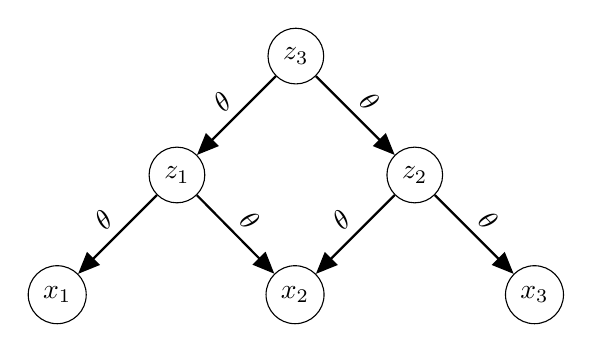
\begin{tikzpicture}
\node[draw, circle] (z3) {$ z_{3} $};

\node[draw, circle, below left =of z3] (z1) {$ z_{1} $};
\node[draw, circle, below right = of z3] (z2) {$ z_{2} $};

\node[draw, circle,  below left= of z1] (in1) {$ x_{1} $};
\node[draw, circle, below left=of z2] (in2) {$ x_{2} $}; 
\node[draw, circle, below right= of z2] (in3) {$ x_{3} $};

\draw[->, thick] (z1) -- (in1) node[midway, above, rotate=45] {$ \theta $};
\draw[->, thick] (z1) -- (in2) node[midway, above, rotate=315] {$ \theta $};
\draw[->, thick] (z2) -- (in2) node[midway, above, rotate=45] {$ \theta $};
\draw[->, thick] (z2) -- (in3) node[midway, above, rotate=315] {$ \theta $};
\draw[->, thick] (z3) -- (z1) node[midway, above, rotate=45] {$ \theta $};
\draw[->, thick] (z3) -- (z2) node[midway, above, rotate=315] {$ \theta $};
\end{tikzpicture}
\end{figure}

\end{frame}

\begin{frame}{Inference Network}

\begin{figure}
\center
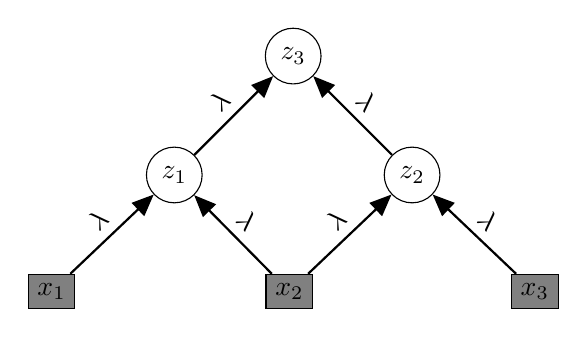
\begin{tikzpicture}
\node[draw, circle] (z3) {$ z_{3} $};

\node[draw, circle, below left =of z3] (z1) {$ z_{1} $};
\node[draw, circle, below right = of z3] (z2) {$ z_{2} $};

\node[draw, rectangle, fill=gray, below left= of z1] (in1) {$ x_{1} $};
\node[draw, rectangle, fill=gray, below left=of z2] (in2) {$ x_{2} $}; 
\node[draw, rectangle, fill=gray, below right= of z2] (in3) {$ x_{3} $};

\draw[->, thick] (in1) -- (z1) node[midway, above, rotate=45] {$ \lambda $};
\draw[->, thick] (in2) -- (z1) node[midway, above, rotate=315] {$ \lambda $};
\draw[->, thick] (in2) -- (z2) node[midway, above, rotate=45] {$ \lambda $};
\draw[->, thick] (in3) -- (z2) node[midway, above, rotate=315] {$ \lambda $};
\draw[->, thick] (z1) -- (z3) node[midway, above, rotate=45] {$ \lambda $};
\draw[->, thick] (z2) -- (z3) node[midway, above, rotate=315] {$ \lambda $};
\end{tikzpicture}
\end{figure}

\end{frame}

\begin{frame}{Wake-sleep Training}
\textbf{Wake Phase} \\
\begin{itemize}
\item Use inference network to sample hidden unit setting $ z $ from $ q(z|x,\lambda) $
\item Update generation parameters $ \theta $ to maximize join log-liklelihood of data and latents $ p(x,z|\theta) $
\end{itemize}
\pause
\textbf{Sleep Phase}
\begin{itemize}
\item Produce dream sample $ \tilde{x} $ from random hidden unit $ z $
\item Update inference parameters $ \lambda $ to maximize probability of latent state $ q(z|\tilde{x},\lambda) $
\end{itemize}
\end{frame}

\begin{frame}{Wake Phase Objective}
Objective  %

\vspace{-15pt}

\begin{equation*}
\begin{aligned}
&\argmin_{\theta} \KL{q(z|x, \lambda)}{p(z|x, \theta)} \\ \pause
&= \argmax_{\theta}~ \underbrace{\mathbb E_{q(z|x, \lambda)}\left[ \log p(z, x| \theta) \right] + \mathbb H[q(z|x, \lambda)]}_{\mathcal G(\theta)}  \pause
\end{aligned}
\end{equation*}
\vspace{-2pt}
Gradient estimate
\begin{equation*}
\begin{aligned}
\grad_\theta \mathcal G(\theta) &= \textcolor{blue}{\grad_\theta}  \mathbb E_{q(z|x, {\lambda})}\left[ \log p(z, x| \textcolor{blue}{\theta}) \right] + \textcolor{blue}{\grad_\theta} \mathbb H[q(z|x, {\lambda})] \\ \pause 
&=\mathbb E_{q(z|x, {\lambda})}\left[ \textcolor{blue}{\grad_\theta} \log p(z, x| \textcolor{blue}{\theta}) \right] \\ \pause
&\overset{\text{MC}}{\approx} \textcolor{blue}{\grad_\theta} \log p(z, x| \textcolor{blue}{\theta}) \quad \textcolor{gray}{\text{where } z \sim q(z|x, \lambda)}
\end{aligned}
\end{equation*} 
 
\end{frame}

\begin{frame}{Wake Phase Objective}

Assumes latent state $ z $ to be fixed random draws from $ q(z|x,\lambda) $.

\begin{equation*}
\begin{aligned}
&\argmin_{\theta} \KL{q(z|x, \lambda)}{p(z|x, \theta)} \\ 
&\overset{\text{MC}}{\approx} \argmax_\theta \log p(z, x| \theta) 
\end{aligned}
\end{equation*} 

This is simply supervised learning with imputed latent data!

\end{frame}


\begin{frame}{Wake Phase Sampling}
Sampling $z \sim q(z|x, \lambda)$
\only<1>{
\begin{figure}
\center
\begin{tikzpicture}
\node[draw, circle] (z3) {$ z_{3} $};

\node[draw, circle, below left =of z3] (z1) {$ z_{1} $};
\node[draw, circle, below right = of z3] (z2) {$ z_{2} $};

\node[draw, rectangle,  below left= of z1] (in1) {$ x_{1} $};
\node[draw, rectangle, below left=of z2] (in2) {$ x_{2} $}; 
\node[draw, rectangle, below right= of z2] (in3) {$ x_{3} $};
\end{tikzpicture}
\end{figure}
}
\only<2>{
\begin{figure}
\center
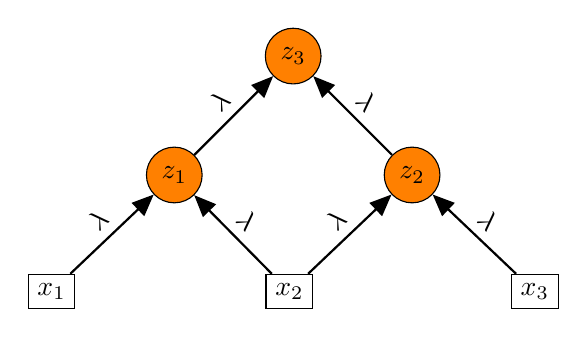
\begin{tikzpicture}
\node[draw, circle, fill=orange] (z3) {$ z_{3} $};

\node[draw, circle, fill=orange, below left =of z3] (z1) {$ z_{1} $};
\node[draw, circle, fill=orange, below right = of z3] (z2) {$ z_{2} $};

\node[draw, rectangle,  below left= of z1] (in1) {$ x_{1} $};
\node[draw, rectangle, below left=of z2] (in2) {$ x_{2} $}; 
\node[draw, rectangle, below right= of z2] (in3) {$ x_{3} $};

\draw[->, thick] (in1) -- (z1) node[midway, above, rotate=45] {$ \lambda $};
\draw[->, thick] (in2) -- (z1) node[midway, above, rotate=315] {$ \lambda $};
\draw[->, thick] (in2) -- (z2) node[midway, above, rotate=45] {$ \lambda $};
\draw[->, thick] (in3) -- (z2) node[midway, above, rotate=315] {$ \lambda $};
\draw[->, thick] (z1) -- (z3) node[midway, above, rotate=45] {$ \lambda $};
\draw[->, thick] (z2) -- (z3) node[midway, above, rotate=315] {$ \lambda $};
\end{tikzpicture}
\end{figure}
}
\end{frame}



\begin{frame}{Wake Phase Update}
\hfill Update $\theta$
\begin{figure}
\center
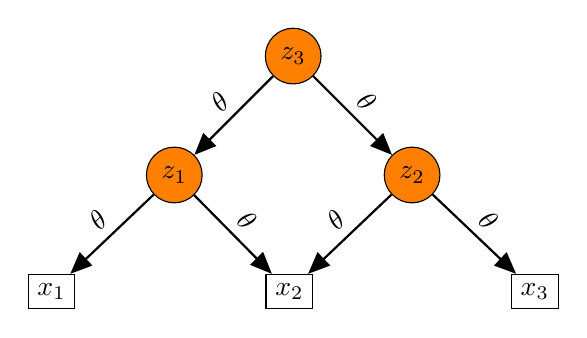
\begin{tikzpicture}
\node[draw, circle, fill=orange] (z3) {$ z_{3} $};

\node[draw, circle, fill=orange, below left =of z3] (z1) {$ z_{1} $};
\node[draw, circle, fill=orange, below right = of z3] (z2) {$ z_{2} $};

\node[draw, rectangle,  below left= of z1] (in1) {$ x_{1} $};
\node[draw, rectangle, below left=of z2] (in2) {$ x_{2} $}; 
\node[draw, rectangle, below right= of z2] (in3) {$ x_{3} $};

\draw[->, thick] (z1) -- (in1) node[midway, above, rotate=45] {$ \theta $};
\draw[->, thick] (z1) -- (in2) node[midway, above, rotate=315] {$ \theta $};
\draw[->, thick] (z2) -- (in2) node[midway, above, rotate=45] {$ \theta $};
\draw[->, thick] (z2) -- (in3) node[midway, above, rotate=315] {$ \theta $};
\draw[->, thick] (z3) -- (z1) node[midway, above, rotate=45] {$ \theta $};
\draw[->, thick] (z3) -- (z2) node[midway, above, rotate=315] {$ \theta $};
\end{tikzpicture}
\end{figure}
\end{frame}


\begin{frame}{Sleep Phase Objective}
Objective  %

\vspace{-15pt}

\begin{equation*}
\begin{aligned}
&\argmin_{\lambda} \KL{q(z|x, \lambda)}{p(z|x, \theta)} \\ \pause
&= \argmax_{\lambda}~ \underbrace{\mathbb E_{q(z|x, \lambda)}\left[ \log p(z, x| \theta) \right] + \mathbb H[q(z|x, \lambda)]}_{\mathcal R(\lambda)}  \pause
\end{aligned}
\end{equation*}

Gradient estimate

\vspace{-10pt}
\begin{equation*}
\begin{aligned}
\grad_\lambda \mathcal R(\lambda) &=  \alert{\grad_\lambda} \mathbb E_{q(z|x, \alert{\lambda})}\left[ \log p(z, x| \theta) \right] + \alert{\grad_\lambda} \alert{\mathbb H[q(z|x, \lambda)]} 
\end{aligned}
\end{equation*} 

\pause

\alert{Let's change the objective!}

\end{frame}


\begin{frame}{Sleep Phase (Convenient) Objective}
Flip the direction of the KL
\begin{small}
\begin{equation*}
\begin{aligned}
&\argmin_{\lambda} \mathbb E_{p(x)}\left[ \KL{p(z|x, \theta)}{q(z|x, \lambda)} \right] \\ \pause
&= \argmin_{\lambda} \mathbb E_{p(x, z|\theta)}\left[ \log p(z|x, \theta) - \log q(z|x, \lambda) \right] \\ \pause
&= \argmax_{\lambda} \underbrace{\mathbb E_{p(x, z|\theta)}\left[ \log q(z|x, \lambda) \right]}_{\mathcal R(\lambda)} - \underbrace{\mathbb E_{p(x,z|\theta)}\left[ \log p(z|x, \theta) \right]}_{\text{constant}}  \pause
%&\overset{\text{MC}}{\approx} \argmax_{\lambda} \log q(z|\tilde{x}, \lambda) 
\end{aligned}
\end{equation*}
\end{small}
\vspace{-3pt}
Gradient 
\vspace{-2pt}
\begin{equation*}
\begin{aligned}
&\grad_\lambda \mathcal R(\lambda) = \textcolor{blue}{\grad_\lambda} \mathbb E_{p(x, z|\theta)}\left[ \log q(z|x, \textcolor{blue}{\lambda}) \right] \\ \pause
&=  \mathbb E_{p(x, z|\theta)}\left[ \textcolor{blue}{\grad_\lambda}  \log q(z|x, \textcolor{blue}{\lambda}) \right]  
 %\overset{\text{MC}}{\approx} \argmax_{\lambda} \log q(z|\tilde{x}, \lambda) \\
\end{aligned}
\end{equation*}
%where $ z \sim p(z)$ and $\tilde{x} \sim p(x|z)$ \hfill \alert{(fake data!)}
\end{frame}

\begin{frame}{Sleep Phase (Convenient) Objective}


Assumes fake data $ \tilde{x} $ and latent variables $ z $ to be fixed random draws from $ p(x,z|\theta) $.
\begin{equation*}
\begin{aligned}
&\argmax_{\lambda}~  \E[p(x, z|\theta)]{\log q(z|x, \lambda)} \pause \\
&\overset{\text{MC}}{\approx} \argmax_{\lambda}~ \log q(z|\tilde x, \lambda)
\end{aligned}
\end{equation*} 

where $ z \sim p(z)$ and $\tilde{x} \sim p(x|z)$ \hfill \alert{(fake data!)}

\end{frame}

\begin{frame}[t]{Sleep Phase Sampling}
Sampling $(z, \tilde x) \sim p(x,z|\theta)$
\only<1>{
\begin{figure}
\center
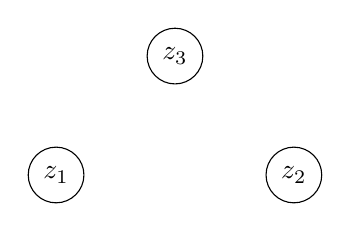
\begin{tikzpicture}
\node[draw, circle] (z3) {$ z_{3} $};

\node[draw, circle, below left =of z3] (z1) {$ z_{1} $};
\node[draw, circle, below right = of z3] (z2) {$ z_{2} $};
\end{tikzpicture}
\end{figure}
}
\only<2>{
\begin{figure}
\center
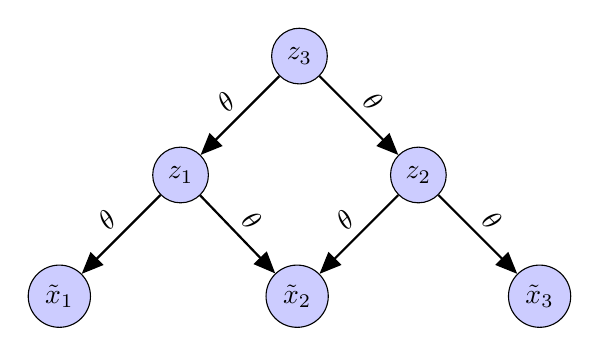
\begin{tikzpicture}
\node[draw, circle, fill=blue!20] (z3) {$ z_{3} $};

\node[draw, circle, fill=blue!20, below left =of z3] (z1) {$ z_{1} $};
\node[draw, circle, fill=blue!20, below right = of z3] (z2) {$ z_{2} $};

\node[draw, circle, fill=blue!20, below left= of z1] (in1) {$ \tilde{x}_{1} $};
\node[draw, circle, fill=blue!20, below left=of z2] (in2) {$ \tilde{x}_{2} $}; 
\node[draw, circle, fill=blue!20, below right= of z2] (in3) {$ \tilde{x}_{3} $};

\draw[->, thick] (z1) -- (in1) node[midway, above, rotate=45] {$ \theta $};
\draw[->, thick] (z1) -- (in2) node[midway, above, rotate=315] {$ \theta $};
\draw[->, thick] (z2) -- (in2) node[midway, above, rotate=45] {$ \theta $};
\draw[->, thick] (z2) -- (in3) node[midway, above, rotate=315] {$ \theta $};
\draw[->, thick] (z3) -- (z1) node[midway, above, rotate=45] {$ \theta $};
\draw[->, thick] (z3) -- (z2) node[midway, above, rotate=315] {$ \theta $};
\end{tikzpicture}
\end{figure}
}
\end{frame}

\begin{frame}[t]{Sleep Phase Update}
\hfill Update $\lambda$
\begin{figure}
\center
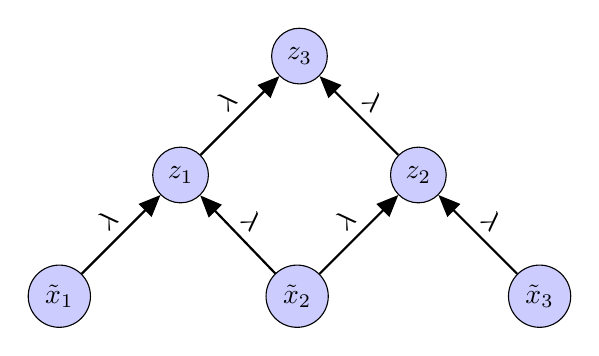
\begin{tikzpicture}
\node[draw, circle, fill=blue!20] (z3) {$ z_{3} $};

\node[draw, circle, fill=blue!20, below left =of z3] (z1) {$ z_{1} $};
\node[draw, circle, fill=blue!20, below right = of z3] (z2) {$ z_{2} $};

\node[draw, circle, fill=blue!20, below left= of z1] (in1) {$ \tilde{x}_{1} $};
\node[draw, circle, fill=blue!20, below left=of z2] (in2) {$ \tilde{x}_{2} $}; 
\node[draw, circle, fill=blue!20, below right= of z2] (in3) {$ \tilde{x}_{3} $};

\draw[->, thick] (in1) -- (z1) node[midway, above, rotate=45] {$ \lambda $};
\draw[->, thick] (in2) -- (z1) node[midway, above, rotate=315] {$ \lambda $};
\draw[->, thick] (in2) -- (z2) node[midway, above, rotate=45] {$ \lambda $};
\draw[->, thick] (in3) -- (z2) node[midway, above, rotate=315] {$ \lambda $};
\draw[->, thick] (z1) -- (z3) node[midway, above, rotate=45] {$ \lambda $};
\draw[->, thick] (z2) -- (z3) node[midway, above, rotate=315] {$ \lambda $};
\end{tikzpicture}
\end{figure}
\end{frame}

\begin{frame}{Wake-sleep Algorithm}
\textbf{Advantages}
\begin{itemize}
\item Simple layer-wise updates
\item Amortised inference: all latent variables are inferred from the same weights $ \lambda $
\end{itemize}
\pause
\textbf{Drawbacks}
\begin{itemize}
\item Inference and generative networks are trained on different objectives
\item Inference weights $ \lambda $ are updated on fake data $ \tilde{x} $
\item Generative weights are bad initially, giving wrong signal to the updates of $ \lambda $
\end{itemize}
\end{frame}


\section{Neural Variational Inference}
\frame{\tableofcontents[currentsection]}



\begin{frame}{Variational Inference Learning (NVIL)}

Generative model with NN likelihood
\pause

~

Let us consider a latent factor model for topic modelling: \pause

\begin{itemize}
	\item a document $ x = (x_{1},\ldots,x_{N})$ consists of $ n $ i.i.d. categorical draws from that model \pause
	\item the categorical distribution in turn depends on  binary latent factors $ z = (z_{1},\ldots,z_{K}) $ which are also i.i.d. 
\end{itemize}


\end{frame}

\begin{frame}{Latent factor model}

\begin{equation*}
\begin{aligned}
Z_{j} &\sim \BerDist{\phi} && (1 \leq k \leq K) \\ 
X_{i}|z &\sim \CatDist{f(z; \theta)} && (1 \leq i \leq N)
\end{aligned}
\end{equation*} 
Here $0 < \phi < 1$ specifies a Bernoulli prior \\
~ and $ f(\cdot; \theta) $ is a function computed by a \\
~ neural network with softmax output, e.g.

\begin{equation*}
\begin{aligned}
f(z; \theta) &= \softmax(Wz + b) \\
\theta &= \{W, b\}
\end{aligned}
\end{equation*}

\end{frame}

\begin{frame}{Example Model}
\begin{figure}
\center
\begin{tikzpicture}
\foreach \x in {1,...,4} {
  \pgfmathtruncatemacro{\y}{\x-1}
  \ifthenelse{\x=1}{\node[obs] (x\x) {$ x_{\x} $}}{\node[obs, right= of x\y] (x\x) {$ x_{\x} $}};
}
\foreach \z in {1,2,3} {
  \node[latent, above right = of x\z] (z\z) {$ z_{\z} $};
  \edge{z\z}{x1,x2,x3,x4};
}
\edge[-,red]{z1}{z2};
\edge[-,red,bend left]{z1}{z3};
\edge[-,red]{z2}{z3};
\end{tikzpicture}
\end{figure}
At inference time the latent variables are marginally dependent. For our variational distribution
we are going to assume that they are not (recall: mean field assumption).
\end{frame}

\begin{frame}{Mean Field Inference}
\begin{figure}
\center
\begin{tikzpicture}
\foreach \x in {1,...,4} {
\pgfmathtruncatemacro{\y}{\x-1}
\ifthenelse{\x=1}{\node[obs] (x\x) {$ x_{\x} $}}{\node[obs, right= of x\y] (x\x) {$ x_{\x} $}};
}
\foreach \z in {1,2,3} {
  \node[latent, above right = of x\z] (z\z) {$ z_{\z} $};
  \edge[color=red]{x1,x2,x3,x4}{z\z};
}
\node[above = of z2] (lambda) {$\lambda$};
\foreach \z in {1,2,3} {
  \edge[color=red]{lambda}{z\z};
}

\end{tikzpicture}
\end{figure}
The inference network needs to predict $ K $ Bernoulli parameters $ b_1^K $. Any neural network with
sigmoid output will do that job.

\end{frame}

\begin{frame}{Inference Network}
\begin{equation*}
\begin{aligned}
	q(z|x, \lambda) &= \prod_{k=1}^K \Bern(z_k|b_k) \\
	&\quad~\text{where }b_1^K = g(x; \lambda)
\end{aligned}
\end{equation*}

Example architecture 
\begin{equation*}
\begin{aligned}
h = \frac{1}{N} \sum_{i=1}^N E_{x_i} \qquad b_1^K = \sigmoid( M h + c)
\end{aligned}
\end{equation*}

$\lambda = \{E, M, c\}$

\end{frame}



\begin{frame}{Objective}

\begin{equation*}
\begin{aligned}
&\ELBO = \E[q(z|x, \lambda)]{\log p(x,z|\theta)} + \Ent{q(z|x, \lambda)} \\ 
&= \E[q(z|x, \lambda)]{\log p(x|z, \theta)} - \KL{q(z|x, \lambda)}{p(z)}
\end{aligned}
\end{equation*}


Parameter estimation
\begin{equation*}
\argmax_{\theta,\lambda} ~ \E[q(z|x,\lambda)]{\log p(x|z,\theta)} - \KL{q(z|x,\lambda)}{p(z)}
\end{equation*}


\end{frame}

\begin{frame}{KL}

KL between $K$ independent Bernoulli distributions is tractable

\begin{equation*}
\begin{aligned}
	&\KL{q(z|x, \lambda)}{p(z|\phi)}  = \sum_{k=1}^K \KL{q(z_k|x, \lambda)}{p(z_k|\phi)} \\
	&=  \sum_{k=1}^K b_k \log \frac{b_k}{\phi} + (1 - b_k) \log \frac{1 - b_k}{1 - \phi}
\end{aligned}
\end{equation*}

\end{frame}

\begin{frame}{Generative Network Gradient}
\begin{equation*}
\begin{aligned}
&\pdv{\theta} \left( \E[q(z|x,\lambda)]{\log p(x|z,\theta)} - \overbrace{\KL{q(z|x,\lambda)}{p(z)}}^{\text{constant wrt }\theta} \right) \\ \pause 
&=\underbrace{\E[q(z|x,\lambda)]{\pdv{\theta}\log p(x|z,\theta)}}_{\text{expected gradient :)}} \\ \pause
&\overset{\text{MC}}{\approx} \frac{1}{S}\sum_{s=1}^{S}
\pdv{\theta} \log p(x|z^{(s)},\theta) \quad \textcolor{gray}{\text{where } z^{(s)} \sim q(z|x,\lambda)}
\end{aligned}
\end{equation*}

\end{frame}

\begin{frame}{Inference Network Gradient}
\begin{equation*}
\begin{aligned}
&\pdv{\lambda}\left(\E[q(z|x,\lambda)]{\log p(x|z,\theta)} - \overbrace{\KL{q(z|x,\lambda)}{p(z)}}^{\text{analytical}} \right) \\ \pause
=&\pdv{\lambda}\E[q(z|x,\lambda)]{\log p(x|z,\theta)} - \underbrace{\pdv{\lambda}\KL{q(z|x,\lambda)}{p(z)}}_{\text{analytical computation}} \\
\end{aligned}
\end{equation*}
\pause
The first term again requires approximation by sampling,  but there is a problem

\end{frame}

\begin{frame}{Inference Network Gradient}
\begin{equation*}
\begin{aligned}
&\pdv{\lambda}\E[q_\lambda(z|x)]{\log p_\theta(x|z)} \\ \pause
&= \pdv{\lambda} \sum_z q(z|x,\lambda)\log p(x|z, \theta)  \\ \pause
&=  \underbrace{\sum_z \alert{\pdv{\lambda}(q(z|x, \lambda))} \log p(x|z, \theta)}_{\text{not an expectation}} 
\end{aligned}
\end{equation*}

\pause

\begin{itemize}
	\item MC estimator is non-differentiable \\ \pause
	\item Differentiating the expression does not yield an expectation: cannot approximate via MC
\end{itemize}

\end{frame}


\section{Score function estimator}

\begin{frame}{Score function estimator}

We can again use the log identity for derivatives
\vspace{-5pt}
\begin{equation*}
\begin{aligned}
&\pdv{\lambda}\E[q_\lambda(z|x)]{\log p_\theta(x|z)} \\ 
%&= \pdv{\lambda} \sum_z q(z|x,\lambda)\log p(x|z, \theta)  \\ 
&=  \sum_z \alert{\pdv{\lambda}(q(z|x, \lambda))} \log p(x|z, \theta) \\  \pause
&= \sum_z \textcolor{blue}{q(z|x, \lambda) \pdv{\lambda}(\log q(z|x, \lambda))} \log p(x|z, \theta)  \\ \pause
&= \underbrace{\mathbb E_{q(z|x, \lambda)} \left[  \log p(x|z, \theta)  \pdv{\lambda}\log q(z|x, \lambda)\right]}_{\text{expected gradient :)}}
\end{aligned}
\end{equation*}


\end{frame}

\begin{frame}{Score function estimator: remarks}


We can now build an MC estimator
\begin{small}
\begin{equation*}
\begin{aligned}
&\pdv{\lambda}\E[q(z|x,\lambda)]{\log p(x|z,\theta)} \\ 
&= \mathbb E_{q(z|x,\lambda)} \left[  \log p(x|z,\theta)  \pdv{\lambda}\log q(z|x,\lambda)\right] \\ \pause 
&\overset{\text{MC}}{\approx} \frac{1}{S} \sum_{s=1}^S \alert{\log p(x|z^{(s)}, \theta)} \pdv{\lambda}\log q(z^{(s)}|x, \lambda) \\
&\textcolor{gray}{\text{where } z^{(s)} \sim q(z|x, \lambda)}
\end{aligned}
\end{equation*}
\end{small}

\pause
\begin{itemize}
	\item magnitude of $\log p(x|z, \theta)$ varies widely \pause 
	\item model likelihood does not contribute to direction of gradient 
\end{itemize}
\end{frame}


\begin{frame}{Computation Graph}
\begin{figure}
\center
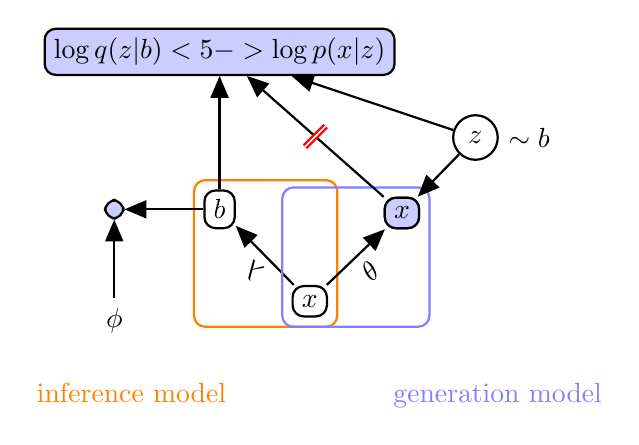
\begin{tikzpicture}[node distance=1cm]

% input
\node[rectangle, draw, rounded corners, thick] (input) {$x$};
% bern parameters
\node[rectangle, draw, rounded corners, thick, above left=of input] (psi) {$ b $};
% x -> b
\draw[->, thick] (input) -- (psi) node[midway, above, rotate=145] {$ \lambda $};
% plate for inference net
\node[draw=orange, thick, rectangle, fit= (input) (psi), rounded corners] {};
\node[below left= of input] (inference) {\textcolor{orange}{inference model}};

\pause

% sample latent variable
\node[above right= of input] (stub) {};
\node[circle, draw, thick, above right= of stub] (z) {$ z $};
\node[right = of z, xshift=-1cm] (random) {$ \sim \BerDist{b} $};

\pause

% log p(x|z)
\node[rectangle, fill=blue!20, thick, above right= of input, rounded corners, draw] (loss) {$ x $};
% x -> log p(x|z)
\draw[->, thick] (input) -- (loss) node[midway, above, rotate=225] {$ \theta $};
% plate for gen net
\node[draw=blue!50, thick, rectangle, fit= (input) (loss), rounded corners] {};
\node[below right= of input] (generation) {\textcolor{blue!50}{generation model}};

\draw[->, thick] (z) edge (loss);


% KL
\pause
\node[rectangle, draw, fill=blue!20, thick, rounded corners, thick, left=of psi] (kl) {$ \KullbackLeibler $};
\node[below= of kl] (phi) {$\phi$ };
\draw[->, thick] (psi) edge (kl);
\draw[->, thick] (phi) edge (kl);



\pause
\node[rectangle, fill=blue!20, thick, above of= psi, rounded corners, draw, node distance=2cm] (scorefunction) {$ \log q(z|b) \uncover<5->{\alert{\log p(x|z)}} $};
\node[rectangle, fill=blue!20, thick, above right= of input, rounded corners, draw] (loss) {$ x $};
\draw[->, thick] (psi) edge (scorefunction);
\draw[->, thick] (z) edge (scorefunction);
\uncover<5->{\draw[->, thick] (loss) edge node[strike out,draw,-,red,double]{} (scorefunction);}

\end{tikzpicture}
\end{figure}
\end{frame}

\begin{frame}{Pros and Cons}
\begin{itemize}
\item Pros
\begin{itemize}
\item Applicable to all distributions
\item Many libraries come with samplers for common distributions
\end{itemize}
\pause
\item Cons
\begin{itemize}
\item High Variance!
\end{itemize}
\end{itemize}
\end{frame}

\section{Variance reduction}
\frame{\tableofcontents[currentsection]}

\begin{frame}{When variance is high we can}

\pause

\begin{itemize}
	\item sample more \\ \pause
	\item use variance reduction techniques (e.g. baselines and control variates)\\ 
\end{itemize}
\end{frame}



\begin{frame}{Control variates}

Suppose we want to estimate $\mathbb E[f(Z)]$ 
\begin{equation*}
\hat f \overset{\text{MC}}{\approx} \frac{1}{S} \sum_{s=1}^S f(z^{(s)})
\end{equation*}
and we know the expected value of another function $\psi(z)$ on the same support. \pause

~

It holds that 

\begin{equation*}
\mathbb E[f(Z)] = \mathbb E[f(Z) - \psi(Z)] + \mathbb E[\psi(Z)]
\end{equation*}


%If $\psi(z) = f(z)$, and we estimate the expected value of $f(x) - \psi(x)$, then we have reduced variance to $0$. \pause 

\end{frame}

\begin{frame}{Variance reduction}
\begin{equation*}
\hat d = \frac{1}{S} \left( \sum_{s=1}^S f(z^{(s)}) - \psi(z^{(s)})\right) + \underbrace{\mathbb E[\psi(Z)]}_{\mu_\psi}
\end{equation*}
In general
\begin{equation*}
\Var(\hat d) = \Var(\hat f) - 2\Cov(\hat f, \hat \psi) + \underbrace{\Var(\mu_\psi)}_{0}
\end{equation*}
If $f$ and $\psi$ are strongly correlated, then we improve on the original estimation problem.


\end{frame}

\begin{frame}{Baselines}
\begin{block}{Fact}
The Expectation of the score function is 0. 
\pause
\begin{equation*}
\E[q(z|x,\lambda)]{\pdv{\lambda} \log q(z|x,\lambda)} = 0
\end{equation*}
\end{block}
\end{frame}

\begin{frame}{Baselines}
We attempt to centre the gradient estimate. To do this we learn a quantity $ C $ that we subtract
from the reconstruction loss.
\begin{equation*}
\E[q(z|\lambda) ]{\log q(z|\lambda) \left( \log p(x|z,\theta) - C \right)}
\end{equation*}
We call $ C $ a baseline. It does not change the expected gradient \citep{Williams:1992}.
\end{frame}

\begin{frame}{Baselines}
 \begin{equation*}
\begin{aligned}
&\E[q(z|\lambda)]{\pdv{\lambda}\log q(z|\lambda) \left( \log p(x|z,\theta) - C \right)} = \pause \\
&\underbrace{\E[q(z|\lambda)]{\pdv{\lambda}\log q(z|\lambda)  \log p(x|z,\theta)}}_{\text{score function gradient}}  -
\pause \\
&\underbrace{\E[q(z|\lambda)]{\pdv{\lambda}\log q(z|\lambda)}}_{0}C
\end{aligned}
\end{equation*}
\end{frame}

\begin{frame}{Baselines}
We can make baselines input-dependent to make them more flexible.
\begin{equation*}
\log q(z|\lambda) \left( \log p(x|z,\theta) - C(x; \omega) \right)
\end{equation*}

\pause

However, baselines may not depend on the random value $ z $! Quantities that may depend on the
random value ($ C(z) $) are called \textbf{control variates}. \\

~

See \cite{PaisleyEtAl:2012, RanganathEtAl:2014,GregorEtAl:2014}.
\end{frame}

\begin{frame}{Baselines}
Baselines are predicted by a regression model (e.g. a neural net). \\

~

The model is trained using 
an $ L_{2} $-loss.
\begin{equation*}
\min_\omega \left(C(x; \omega) - \log p(x|z,\theta)\right)^{2}
\end{equation*}
\end{frame}






\begin{frame}{Summary}
\begin{itemize}
\item Wake-Sleep: train inference and generation networks with separate objectives
\pause
\item NVIL: a single objective (ELBO) for both models\\ \pause
\item Use score function estimator\\ 
\pause
\item Always use baselines for variance reduction!
\end{itemize}
\end{frame}

\begin{frame}[allowframebreaks]{Literature}
%\nocite{KingmaWelling:2013}
\nocite{HintonEtAl:1995}
\nocite{MnihNVIL}
\nocite{greensmith2004variance}
%\nocite{RezendeEtAl:2014}
%\nocite{TitsiasLazarogredilla:2014}
%\nocite{BergkirkpatrickEtAl:2010}
%\nocite{KucukelbirEtAl:2017}

\bibliographystyle{plainnat}
\bibliography{../../VI}
\end{frame}

\end{document}